\documentclass[]{article}
\usepackage{polski}
\usepackage[utf8]{inputenc}
\usepackage{amsmath}
\usepackage{mathtools,leftidx}% http://ctan.org/pkg/{mathtools,leftidx}
\usepackage{graphicx}
\usepackage{geometry}
\usepackage{float}

\geometry{legalpaper, margin=0.6in}
\newcommand\T{\mathcal{T}}

%opening
\title{Projekt MORO}
\author{Jakub Postępski}
\date{3 stycznia 2019}

\begin{document}

\maketitle

\section{Robot}
Robot to ABB IRB 7600.

\begin{figure}[H]
	\centering
	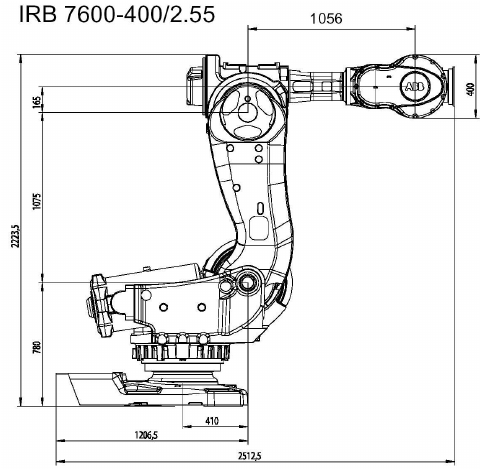
\includegraphics[width=0.95\textwidth]{7600.png}
	\caption{Robot ABB IRB 7600-400 z zaznaczonymi osiami}
	\label{img:irb7600}
\end{figure}

\section{Parametry DH}

\begin{table}[H]
	\begin{tabular}{|| c | c c c c ||}
		\hline
		L. p. & $a_{i-1}$ & $\alpha_{i-1}$ & $d_i$ & $\theta_i$ \\ 
		\hline\hline
		1 & $ 0 $ & $0$ & 0 & $\theta_1$ \\
		\hline
		2 & $a_1$ & $\pi/2$ & 0 & $\theta_2$ \\
		\hline
		3 & $a_2$ & $0$ & 0 & $\theta_3$ \\
		\hline
		4 & $a_3$ & $\pi/2$ & $a_4$ & $\theta_4$ \\
		\hline
		5 & $0$ & $\pi/2$ & 0 & $\theta_5$ \\
		\hline
		6 & $0$ & $\pi/2$ & 0 & $\theta_6$ \\
		\hline
		
	\end{tabular}
	\caption{Parametry DH}
	\label{tab1}
\end{table}

Wartości parametrów:
\[\begin{array}{l}
a_1 = 410 mm \\
a_2 = 1075 mm \\
a_3 = 165 mm \\
d_4 = 1056 mm
\end{array}\]

\section{Kinematyka prosta}
Przejścia pomiędzy członami:
\[\prescript{0}{1}{T}=\begin{bmatrix}
\begin{array}{cccc}
c_1 & -s_1 & 0 & 0 \\
s_1 & c_1 & 0 & 0 \\
0 & 0 & 0 & 0 \\
0 & 0 & 0 & 1 \\
\end{array}
\end{bmatrix}
\]
\[\prescript{1}{2}{T}=\begin{bmatrix}
\begin{array}{cccc}
c_2 & -s_2 & 0 & a_1 \\
0 & 0 & -1 & 0 \\
s_2 & c_2 & 0 & 0 \\
0 & 0 & 0 & 1 \\
\end{array}
\end{bmatrix}
\]
\[\prescript{2}{3}{T}=\begin{bmatrix}
\begin{array}{cccc}
c_3 & -s_3 & 0 & a_2 \\
s_3 & c_3 & 0 & 0 \\
0 & 0 & 1 & 0 \\
0 & 0 & 0 & 1 \\
\end{array}
\end{bmatrix}
\]
\[\prescript{3}{4}{T}=\begin{bmatrix}
\begin{array}{cccc}
c_4 & -s_4 & 0 & a_3 \\
0 & 0 & -1 & -d_4 \\
s_4 & c_4 & 0 & 0 \\
0 & 0 & 0 & 1 \\
\end{array}
\end{bmatrix}
\]

\[\prescript{4}{5}{T}=\begin{bmatrix}
\begin{array}{cccc}
c_5 & -s_5 & 0 & 0 \\
0 & 0 & -1 & 0 \\
s_5 & c_5 & 0 & 0 \\
0 & 0 & 0 & 1 \\
\end{array}
\end{bmatrix}
\]

\[\prescript{5}{6}{T}=\begin{bmatrix}
\begin{array}{cccc}
c_6 & -s_6 & 0 & 0 \\
0 & 0 & -1 & 0 \\
s_6 & c_6 & 0 & 0 \\
0 & 0 & 0 & 1 \\
\end{array}
\end{bmatrix}
\]

Po wymnożeniu:
\[\prescript{0}{6}{T}=\begin{bmatrix}
\begin{array}{cccc}
r_{11} & r_{12} & r_{13} & p_x \\
r_{21} & r_{22} & r_{23} & p_y \\
r_{31} & r_{32} & r_{33} & p_z \\
0 & 0 & 0 & 1 \\
\end{array}
\end{bmatrix}
\]
gdzie:
\[ r_{11} = c_1(c_{23}(c_4c_5c_6 + s_4s_6) + s_{23}s_5c_6) - s_1(c_4s_6 -s_4c_5c_6)\]
\[ r_{12} = c_1(c_{23}(s_4c_6 - c_4c_5c_6) - s_{23}s_5s_6) - s_1(s_4c_5s_6 + c_4s_6)\]
\[ r_{13} = c_1(c_{23}c_4s_5) + s_1s_4s_5\]
\[ r_{21} = s_1(c_{23}(c_4c_5c_6 + s_4s_6) + s_{23}s_5c_6) + c_1(c_4s_6 -s_4c_5c_6 )\]
\[ r_{22} = s_1(c_{23}(s_4c_6 - c_4c_5c_6) - s_{23}s_5s_6) + c_1(s_4c_5s_6 + c_4c_6)\]
\[ r_{23} = s_1(c_{23}c_4s_5 - s_{23}c_5) - c_1s_4s_5\]
\[ r_{31} = s_{23}(c_4c_5c_6 + s_4s_6) - c_{23}s_5c_6\]
\[ r_{32} = s_{23}(s_4c_6 - c_4c_5c_6) + c_{23}s_5s_6\]
\[ r_{33} = s_{23}c_4s_5 + c_{23}c_5\] 
\[ p_x = c_1(c_{23}a_3 + s_{23}d_4 + c_2a_2 + a_1))\] 
\[ p_y = s_1(c_{23}a_3 + s_{23}d_4 + c_2a_2 + a_1))\]
\[ p_z = s_{23}a_3 - c_{23}d_4 + s_2a_2 \]

\section{Kinematyka odwrotna}
Tworzymy dodatkową macierz pośrednią:
\scriptsize
\[\prescript{1}{6}{\T} = \begin{bmatrix}
s_4s_6c_{23} + c_6(s_5s_{23} + c_4c_5c_{23}) &
s_4c_6c_{23} - s_6(s_5s_{23} + c_4c_5c_{23}) &
c_4s_5c_{23} - c_5s_{23} &
a_1 + a_2c_2 + a_3c_{23} + d_4s_{23}
\\
c_4s_6 - c_5c_6s_4 &
c_4c_6 + c_5s_4s_6 &
- s_4s_5 &
0
\\
s_4s_6s_{23} - c_6(s_5c_{23} - c_4c_5s_{23}) &
c_6s_4s_{23} + s_6(s_5c_{23} - c_4c_5s_{23}) &
c_4s_5s_{23} + c_5c_{23} &
a_2s_2 + a_3s_{23} - d_4c_{23}
\\
0 & 0 & 0 & 1
\end{bmatrix}\]
\normalsize

możemy wyprowadzić:
\begin{align*}
\prescript{0}{1}{\T}^{-1} \cdot \prescript{0}{6}{\T}_d &= \\
&= \begin{bmatrix}
c_1 & s_1 & 0 & 0 \\
-s_1 & c_1 & 0 & 0 \\
0 & 0 & 1 & 0 \\
0 & 0 & 0 & 1
\end{bmatrix}\begin{bmatrix}
r_{11} & r_{12} & r_{13} & p_x \\
r_{21} & r_{22} & r_{23} & p_y \\
r_{31} & r_{32} & r_{33} & p_z \\
0 & 0 & 0 & 1
\end{bmatrix} \\
&= \begin{bmatrix}
c_1r_{11} + s_1r_{21} & c_1r_{12} + s_1r_{22} & c_1r_{13} + s_1r_{23} & c_1p_x + s_1p_y \\
c_1r_{21} - s_1r_{11} & c_1r_{22} - s_1r_{12} & c_1r_{23} - s_1r_{13} & c_1p_y - s_1p_x \\
r_{31} & r_{32} & r_{33} & p_z \\
0 & 0 & 0 & 1
\end{bmatrix} \\
&= \prescript{1}{6}{\T}
\end{align*}

\subsection{Stopień 1 ($\theta_1$)}
Bierzemy równanie z $\prescript{1}{6}{\T}_{24}$:
\[\begin{array}{l}
c_1p_y - s_1p_x = 0 \\
\cfrac{s_1}{c_1} = \cfrac{p_y}{p_x} \\
\theta_1 = \arctan \cfrac{p_y}{p_x}
\end{array}\]

\subsection{Stopień 2 ($\theta_2$)}
Bierzemy równania z $\prescript{1}{6}{\T}_{14}$ i $\prescript{1}{6}{\T}_{34}$:

\[\left\{\begin{array}{l}
a_1 + a_2c_2 + a_3c_{23} + d_4s_{23} = c_1p_x + s_1p_y \\
a_2s_2 + a_3s_{23} - d_4c_{23} = p_z
\end{array}\right.\]

i wprowadzając stałe:
\[\left\{\begin{array}{l}
E = c_1p_x + s_1p_y - a_1 \\
F = p_z
\end{array}\right.\]

otrzymujemy:
\[\left\{\begin{array}{l}
a_3c_{23} + d_4s_{23} = E - a_2c_2 \\
a_3s_{23} - d_4c_{23} = F - a_2s_2
\end{array}\right.\]
\[\left\{\begin{array}{l}
(a_3c_{23})^2 + 2a_3d_4c_{23}s_{23} + (d_4s_{23})^2 = E^2 - 2Ea_2c_2 + (a_2c_2)^2 \\
(a_3s_{23})^2 - 2a_3d_4s_{23}c_{23} + (d_4c_{23})^2 = F^2 - 2Fa_2s_2 + (a_2s_2)^2
\end{array}\right.\]

dodając stronami i przekształcając dalej:
\[
a_3^2 + d_4^2 = E^2 + F^2 - 2Ea_2c_2 - 2Fa_2s_2 + a_2^2
\]

podstawiając:
\[
K = E^2 + F^2 + a_2^2 - a_3^2 - d_4^2
\]

oraz stosując współrzędne biegunowe:
\[\left\{\begin{array}{l}
2Ea_2 = Rs_\omega \\
2Fa_2 = Rc_\omega
\end{array}\right.\]

otrzymujemy:
\[\begin{array}{l}
R = \sqrt{4E^2a_2^2 + 4F^2a_2^2} \\
K = 2Ea_2c_2 + 2Fa_2s_2 = Rs_\omega c_2 + Rc_\omega s_2
\end{array}\]

stosując wzór na sumę sinusów oraz jedynkę trygonometryczną:
\[\begin{array}{l}
K = R\sin(\theta_2 + \omega) \\
\sin(\theta_2 + \omega) = \frac{K}{R} \\
\cos(\theta_2 + \omega) = \pm \sqrt{1 - \big(\frac{K}{R}\big)^2}
\end{array}\]

zatem:
\[\begin{array}{l}
\tan(\theta_2 + \omega) = \cfrac{\frac{K}{R}}{\pm \sqrt{1 - \big(\frac{K}{R}\big)^2}} \\
\theta_2 + \omega = \arctan{\cfrac{\frac{K}{R}}{\pm \sqrt{1 - \big(\frac{K}{R}\big)^2}}} \\
\theta_2  = \arctan{\cfrac{\frac{K}{R}}{\pm \sqrt{1 - \big(\frac{K}{R}\big)^2}}} - \arctan{\cfrac{2Ea_2}{2Fa_2}} \\
\end{array}\]

\subsection{Stopień 3 ($\theta_3$)}
Wykorzystujemy równania z poprzedniej sekcji:
\[\left\{\begin{array}{l}
a_3c_{23} + d_4s_{23} = E - a_2c_2 \\
a_3s_{23} - d_4c_{23} = F - a_2s_2
\end{array}\right.\]

należy podstawić:
\[\left\{\begin{array}{l}
M = E - a_2c_2 \\
N = F - a_2s_2
\end{array}\right.\]

i uzyskujemy:
\[\left\{\begin{array}{l}
a_3c_{23} + d_4s_{23} = M \\
a_3s_{23} - d_4c_{23} = N
\end{array}\right.\]

przekształcając dalej:
\[\begin{array}{l}
c_{23} = \cfrac{M - d_4s_{23}}{a_3} \\
a_3s_{23} - d_4\cfrac{M - d_4s_{23}}{a_3} = N \\
a_3^2s_{23} - d_4(M - d_4s_{23}) = Na_3 \\
s_{23} = \cfrac{Na_3 + Md_4}{a_3^2 + d_4^2} \\
c_{23} = \cfrac{M - d_4(\cfrac{Na_3 + Md_4}{a_3^2 + d_4^2})}{a_3}
\end{array}\]

dzieląc $s_{23}$ i $c_{23}$ przez siebie otrzymujemy
\[\begin{array}{l}
\tan(\theta_2 + \theta_3) = \cfrac{s_{23}}{c_{23}} = \cfrac{\cfrac{Na_3 + Md_4}{a_3^2 + d_4^2}}{\cfrac{M - d_4(\frac{Na_3 + Md_4}{a_3^2 + d_4^2})}{a_3}} \\
\tan(\theta_2 + \theta_3) = \cfrac{a_3(Na_3 + Md_4)}{M(a_3^2 + d_4^2) - d_4(Na_3 + Md_4)} \\
\end{array}\]

oraz finalnie:
\[
\theta_3 = \arctan{\cfrac{a_3(Na_3 + Md_4)}{M(a_3^2 + d_4^2) - d_4(Na_3 + Md_4)}} - \theta_2
\]

\subsection{Stopień 4 ($\theta_4$)}
Wykorzystując równanie z $\prescript{1}{6}{\T}_{23}$:
\[
- s_4s_5 = c_1r_{23} - s_1r_{13}
\]

zakładając, że $s_5 \neq 0$ z jedynki trygonometrycznej
\[\begin{array}{l}
s_4 = \cfrac{c_1r_{23} - s_1r_{13}}{s_5} \\
c_4 = \pm \sqrt{1 - \big(\cfrac{c_1r_{23} - s_1r_{13}}{s_5}\big)^2} \\
\tan(\theta_4) = \cfrac{\cfrac{c_1r_{23} - s_1r_{13}}{s_5}}{\pm \sqrt{1 - \big(\cfrac{c_1r_{23} - s_1r_{13}}{s_5}\big)^2}}
\end{array}\]

stąd:
\[
\theta_4 = \arctan\cfrac{\cfrac{c_1r_{23} - s_1r_{13}}{s_5}}{\pm \sqrt{1 - \big(\cfrac{c_1r_{23} - s_1r_{13}}{s_5}\big)^2}}
\]

\subsection{Stopień 5 ($\theta_5$)}
Biorąc równania z $\prescript{1}{6}{\T}_{13}$ i $\prescript{1}{6}{\T}_{33}$:

\[\left\{\begin{array}{l}
c_4s_5c_{23} - c_5s_{23} = c_1r_{13} + s_1r_{23} \\
c_4s_5s_{23} + c_5c_{23} = r_{33}
\end{array}\right.\]

i wprowadzając stałe
\[\left\{\begin{array}{l}
P = c_1r_{13} + s_1r_{23} \\
Q = r_{33}
\end{array}\right.\]

otrzymujemy
\[\left\{\begin{array}{l}
c_4s_5c_{23} - c_5s_{23} = P \\
c_4s_5s_{23} + c_5c_{23} = Q
\end{array}\right.\]

przekształcając dalej:
\[\begin{array}{l}
c_4s_5 = \cfrac{Q - c_5c_{23}}{s_{23}} \\
c_{23}\cfrac{Q - c_5c_{23}}{s_{23}} - c_5s_{23} = P \\
c_{23}(Q - c_5c_{23}) - c_5s_{23}^2 = Ps_{23} \\
c_5(c_{23}^2 + s_{23}^2) = Qc_{23} - Ps_{23} \\
c_5 = Qc_{23} - Ps_{23}
\end{array}\]

z jedynki trygonometrycznej:
\[\begin{array}{l}
s_5 = \pm \sqrt{1 - (Qc_{23} - Ps_{23})^2} \\
\tan(\theta_5) = \cfrac{\pm \sqrt{1 - (Qc_{23} - Ps_{23})^2}}{Qc_{23} - Ps_{23}}
\end{array}\]

i finalnie:
\[
\theta_5 = \arctan\cfrac{\pm \sqrt{1 - (Qc_{23} - Ps_{23})^2}}{Qc_{23} - Ps_{23}}
\]
(Wartości $c_{23}$ oraz $s_{23}$ wyznaczone zostały podczas wyznaczania $\theta_3$).

\subsection{Stopień 6 ($\theta_6$)}
Biorąc równania z $\prescript{1}{6}{\T}_{21}$ i $\prescript{1}{6}{\T}_{22}$:

\[\left\{\begin{array}{l}
c_4s_6 - c_5c_6s_4 = c_1r_{21} - s_1r_{11} \\
c_4c_6 + c_5s_4s_6 = c_1r_{22} - s_1r_{12}
\end{array}\right.\]

i wprowadzając stałe
\[\left\{\begin{array}{l}
S = c_1r_{21} - s_1r_{11} \\
T = c_1r_{22} - s_1r_{12}
\end{array}\right.\]

i uzyskujemy:
\[\left\{\begin{array}{l}
c_4s_6 - c_5c_6s_4 = S \\
c_4c_6 + c_5s_4s_6 = T
\end{array}\right.\]

zakładając $s_5 \neq 0$ i przekształcając:
\[\begin{array}{l}
s_6 = \cfrac{S + c_5c_6s_4}{c_4} \\
c_4c_6 + c_5s_4\cfrac{S + c_5c_6s_4}{c_4} = T \\
c_4^2c_6 + c_5s_4(S + c_5c_6s_4) = Tc_4 \\
c_6 = \cfrac{Tc_4 - Sc_5s_4}{s_4^2c_5^2 + c_4^2}
\end{array}\]

z jedynki trygonometrycznej:
\[\begin{array}{l}
s_6 = \pm \sqrt{1 - (\cfrac{Tc_4 - Sc_5s_4}{s_4^2c_5^2 + c_4^2})^2} \\
\tan(\theta_6) = \cfrac{\pm \sqrt{1 - (\cfrac{Tc_4 - Sc_5s_4}{s_4^2c_5^2 + c_4^2})^2}}{\cfrac{Tc_4 - Sc_5s_4}{s_4^2c_5^2 + c_4^2}}
\end{array}\]

i finalnie:
\[
\theta_6 = \arctan\cfrac{\pm \sqrt{1 - (\cfrac{Tc_4 - Sc_5s_4}{s_4^2c_5^2 + c_4^2})^2}}{\cfrac{Tc_4 - Sc_5s_4}{s_4^2c_5^2 + c_4^2}}
\]

\subsection{Osobliwość $s_5 = 0 \Rightarrow \theta_5 = 0$}
Upraszcza się układ równań dzięki podstawieniom:
\[\begin{array}{l}
s_5 = 0 \\
c_5 = 1
\end{array}\]

więc mamy:
\[\prescript{0}{1}{\T}^{-1} \cdot \prescript{0}{6}{\T}_d = \prescript{1}{6}{\T^*} = \begin{bmatrix}
s_4s_6c_{23} + c_4c_6c_{23} &
s_4c_6c_{23} - c_4s_6c_{23} &
- s_{23} &
a_1 + a_2c_2 + a_3c_{23} + d_4s_{23}
\\
c_4s_6 - s_4c_6 &
c_4c_6 + s_4s_6 &
0 &
0
\\
s_4s_6s_{23} + c_4c_6s_{23} &
c_6s_4s_{23} - c_4s_6s_{23} &
c_{23} &
a_2s_2 + a_3s_{23} - d_4c_{23}
\\
0 & 0 & 0 & 1
\end{bmatrix}\]

można wtedy wykorzystać równania $\prescript{1}{6}{\T^*}_{21}$ i $\prescript{1}{6}{\T^*}_{22}$:
\[\left\{\begin{array}{l}
c_4s_6 - s_4c_6 = c_1r_{21} - s_1r_{11} \\
c_4c_6 + s_4s_6 = c_1r_{22} - s_1r_{12}
\end{array}\right.\]

korzystając ze wzorów na sinus i cosinus sumy:
\[\left\{\begin{array}{l}
\sin(\theta_6 - \theta_4) = c_1r_{21} - s_1r_{11} \\
\cos(\theta_6 - \theta_4) = c_1r_{22} - s_1r_{12}
\end{array}\right.\]

stąd:
\[
\theta_6 - \theta_4 = \arctan\cfrac{c_1r_{21} - s_1r_{11}}{c_1r_{22} - s_1r_{12}}
\]

\end{document}